\section{Техническое задание}

\subsection{Основание для разработки}

Основанием для разработки является задание на выпускную квалификационную работу бакалавра по теме «Информационная система на платформе 1С:Предприятие 8.3 для комплексного учета деятельности спортивной организации».

\subsection{Цель и назначение разработки}

Целью разработки является создание информационной системы на платформе «1С:Предприятие 8.3», предназначенной для комплексного учета деятельности спортивной организации и обеспечения удобного доступа к информации для различных категорий пользователей.

Для достижения указанной цели система должна охватывать как пользовательские сценарии (просмотр расписания, спортсменов, результатов соревнований), так и административные сценарии (ведение справочников, оформление документов, формирование отчетов).

\subsection{Требования к функциональности}

Информационная система должна обеспечивать выполнение следующих функций.

\begin{enumerate}
	\item \textbf{Управление данными о спортсменах и тренерах.} Система должна предоставлять возможность ведения справочников спортсменов и тренеров, включая добавление новых записей, редактирование существующих и удаление. Для каждого спортсмена должны поддерживаться анкетные данные (фамилия, имя, отчество, дата рождения, пол, адрес, телефон, e-mail, дата зачисления) и табличная часть с видами спорта и присвоенными разрядами. Для каждого тренера должны поддерживаться анкетные данные, должность, специализация по виду спорта и даты приема на работу и увольнения.
	
	\item \textbf{Составление и ведение расписания занятий.} Система должна обеспечивать создание документа «Расписание занятий» на календарный месяц с возможностью заполнения табличной части, содержащей сведения о тренере, группе, месте проведения и временных интервалах для каждого дня недели. Временные интервалы выбираются из предварительно заполненного справочника «Периоды времени». При проведении документ должен автоматически формировать записи в регистрах сведений для последующего использования в отчетах.
	
	\item \textbf{Управление соревнованиями.} Система должна предоставлять возможность регистрации соревнований с указанием названия, вида спорта, статуса, дат и места проведения, главного судьи. Документ должен содержать три табличные части: «Дисциплины» (перечень дисциплин с указанием возрастной категории), «Участники» (список спортсменов или команд с указанием дисциплины) и «Судьи» (состав судейской коллегии с указанием роли каждого судьи).
	
	\item \textbf{Учет результатов соревнований.} Система должна обеспечивать ввод результатов участников по каждой дисциплине с указанием результата, занятого места, выполненного разряда и тренера. Документ должен создаваться на основании документа «Соревнования». Должна поддерживаться возможность заполнения табличной части из внешнего файла формата Excel.
	
	\item \textbf{Оформление заявок и приказов на присвоение разрядов.} Система должна поддерживать формирование заявки на присвоение разряда (с указанием вида спорта, желаемого разряда и списка спортсменов) и итогового приказа. Приказ должен иметь печатную форму официального документа.
	
	\item \textbf{Складской учет спортивного инвентаря.} Система должна обеспечивать оформление четырех видов складских документов: поступление, выдача, возврат и списание инвентаря. При проведении документы должны автоматически формировать движения по регистру накопления «Спортивный инвентарь организации», что позволяет в любой момент получить актуальные остатки инвентаря в разрезе материально-ответственных лиц.
	
	\item \textbf{Формирование отчетности.} Система должна предоставлять следующие отчеты: «Расписание занятий общее» (календарный вид с группировкой по видам спорта и тренерам), «Расписание занятий группы» (расписание для выбранной группы), «Расписание занятий тренера» (расписание для конкретного тренера), «Список спортсменов» (с группировкой по видам спорта и тренерам), «Результаты соревнований» (с детализацией по соревнованиям и дисциплинам).
	
	\item \textbf{Разграничение доступа.} Система должна обеспечивать разделение прав пользователей на основе ролей: администратор (полный доступ ко всем функциям, включая управление пользователями и настройку почтовых оповещений) и тренер (просмотр расписания, спортсменов, групп; внесение и редактирование результатов соревнований; формирование отчетов по расписанию; без доступа к складским документам, приказам и настройкам системы).
	
	\item \textbf{Отправка уведомлений.} Система должна обеспечивать возможность отправки уведомлений участникам соревнований по электронной почте с использованием предварительно настроенной учетной записи.
\end{enumerate}

\subsection{Требования к интерфейсу}

Интерфейс информационной системы представляет собой управляемое приложение 1С:Предприятие, организованное по принципу функциональных подсистем. Такой подход обеспечивает логичную группировку команд и объектов, интуитивно понятную навигацию и снижение порога входа для новых пользователей.

Система должна включать следующие подсистемы:

\begin{itemize}
	\item «Учет спортсменов и тренеров» (справочники, кадровые документы и приказы);
	\item «Учет соревнований» (справочники судей, документы соревнований и результатов);
	\item «Учет спортивного инвентаря» (справочники инвентаря и складские документы);
	\item «Администрирование» (настройка учетных записей почты и управление пользователями).
\end{itemize}

Все формы документов и справочников должны быть выполнены в едином стиле управляемого приложения. Каждая форма документа должна содержать командную панель с кнопками «Провести и закрыть», «Записать», «Провести», а также дополнительные команды, специфичные для конкретного документа: «Печать», «Вложенные файлы», «Создать на основании», «Заполнить из файла», «Отправить напоминание по эл. почте».

Для визуализации расписания занятий должен использоваться элемент управления «Планировщик», позволяющий отображать расписание в календарном виде с группировкой по видам спорта, тренерам и группам.

\subsection{Моделирование вариантов использования}

В системе выделяются два действующих лица.

\begin{enumerate}
	\item Администратор - управляет всеми данными системы, оформляет документы, формирует отчеты, настраивает параметры системы.
	\item Тренер - просматривает расписание, списки групп и спортсменов, вносит результаты соревнований.
\end{enumerate}


На рисунке 2.1 представлена диаграмма прецедентов для роли «Администратор».

\begin{center}
	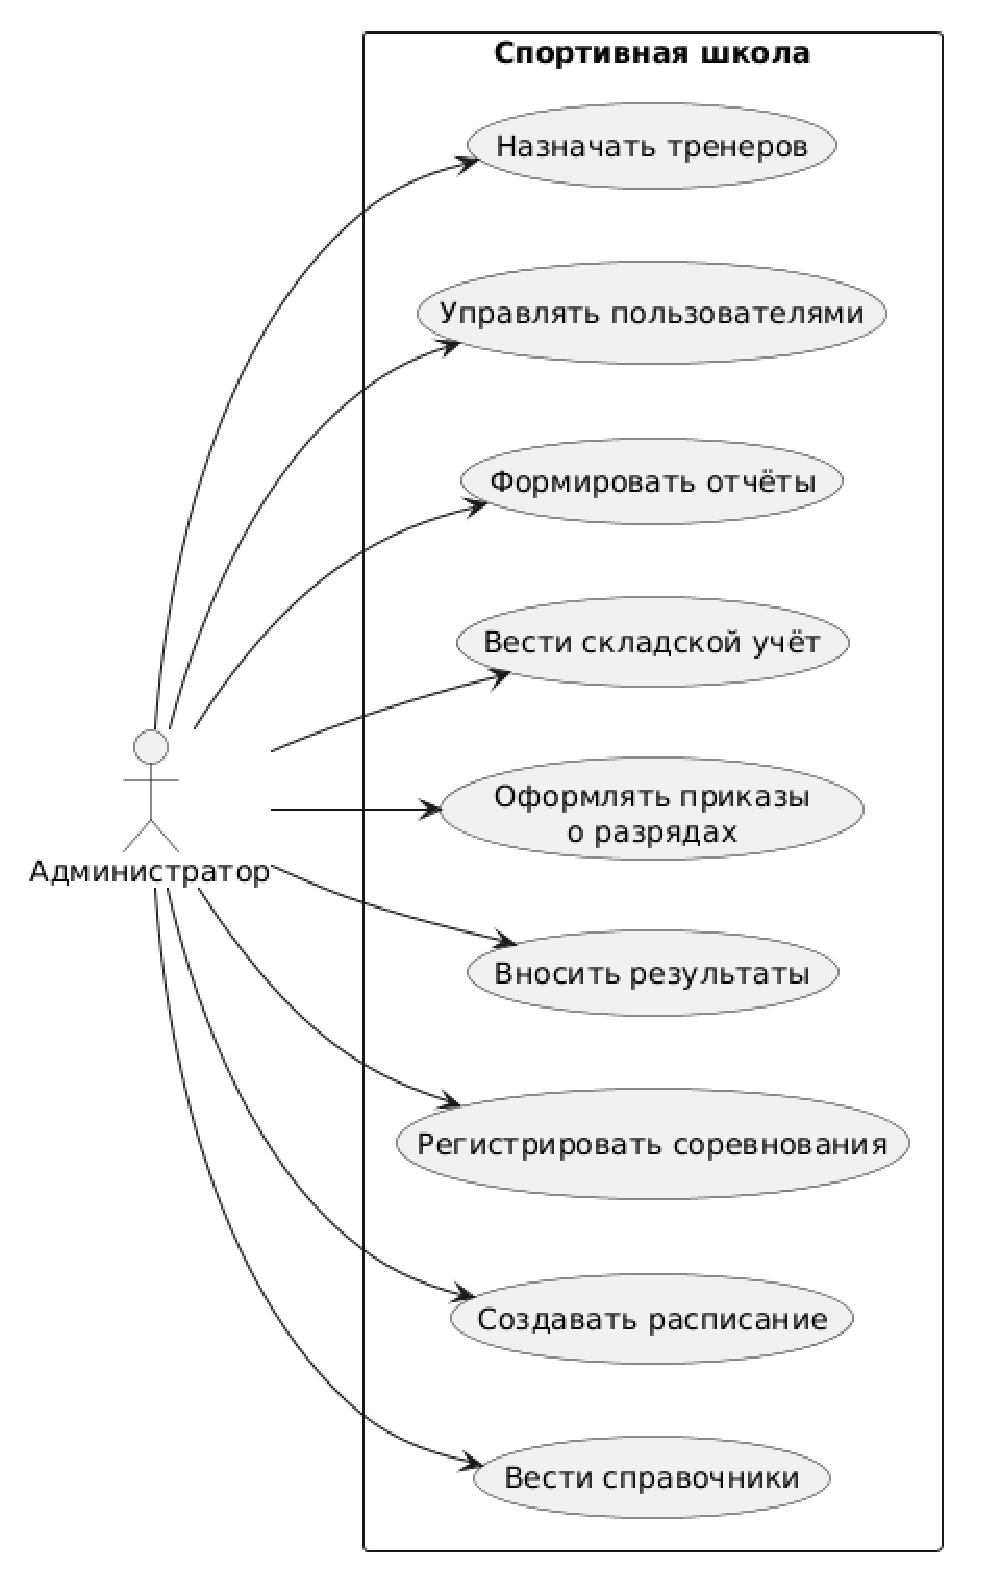
\includegraphics[width=0.9\textwidth]{images/diagramma_admin2.eps}
\end{center}
\begin{center}
	Рисунок 2.1 - Диаграмма прецедентов для администратора
\end{center}

На рисунке 2.2 представлена диаграмма прецедентов для роли «Тренер».

\begin{center}
	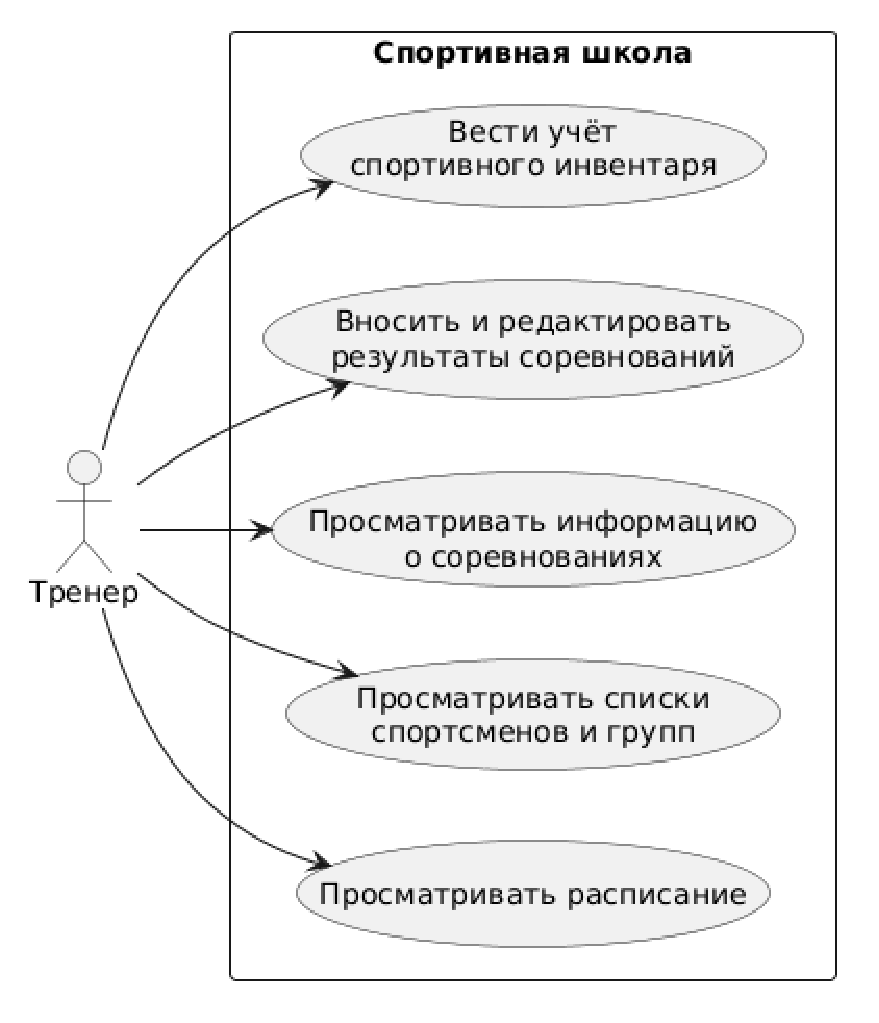
\includegraphics[width=0.9\textwidth]{images/diagramma_trener.eps}
\end{center}
\begin{center}
	Рисунок 2.2 - Диаграмма прецедентов для тренера
\end{center}

\vspace{0.3cm}

 Далее приведены детальные варианты использования для каждой роли, оформленные в виде текстовых сценариев.

\subsubsection{Вариант использования «Ведение справочника спортсменов»}

\textbf{Заинтересованные лица и их требования:} администратор желает поддерживать в актуальном состоянии список спортсменов школы.

\textbf{Предусловие:} открыт справочник «Спортсмены».

\textbf{Постусловие:} изменения сохранены в базе данных.

\textbf{Основной успешный сценарий:}

\begin{enumerate}
	\item Администратор открывает справочник «Спортсмены».
	\item Система отображает список всех спортсменов.
	\item Администратор нажимает «Создать» для добавления нового спортсмена.
	\item Система открывает форму элемента справочника.
	\item Администратор заполняет обязательные поля (фамилия, имя, отчество, дата рождения) и табличную часть с видами спорта и разрядами.
	\item Администратор нажимает «Записать и закрыть».
	\item Система сохраняет запись и обновляет список.
\end{enumerate}

\subsubsection{Вариант использования «Создание расписания занятий»}

\textbf{Заинтересованные лица и их требования:} администратор желает составить расписание тренировок на месяц.

\textbf{Предусловие:} открыт список документов «Расписание занятий».

\textbf{Постусловие:} документ проведен, записи в регистрах сформированы.

\textbf{Основной успешный сценарий:}

\begin{enumerate}
	\item Администратор создает новый документ «Расписание занятий».
	\item Система автоматически присваивает номер и устанавливает текущую дату.
	\item Администратор указывает месяц, на который составляется расписание.
	\item Администратор добавляет строки в табличную часть: выбирает тренера, группу, место проведения и указывает временные интервалы для каждого дня недели.
	\item Администратор нажимает «Провести и закрыть».
	\item Система проверяет заполнение обязательных полей.
	\item Документ проводится, формируются записи в регистрах сведений.
	\item Система закрывает форму документа.
\end{enumerate}

\textbf{Альтернативный сценарий (не заполнены обязательные поля):}

\begin{enumerate}
	\item Администратор не заполняет поле «Месяц» или не добавляет ни одной строки в табличную часть.
	\item Администратор нажимает «Провести и закрыть».
	\item Система выводит сообщение об ошибке: «Не заполнены обязательные реквизиты».
	\item Документ не проводится, форма остается открытой для исправления.
\end{enumerate}

\subsubsection{Вариант использования «Регистрация соревнования»}

\textbf{Заинтересованные лица и их требования:} администратор желает зарегистрировать новое соревнование.

\textbf{Предусловие:} открыт список документов «Соревнования».

\textbf{Постусловие:} соревнование зарегистрировано в системе.

\textbf{Основной успешный сценарий:}

\begin{enumerate}
	\item Администратор создает новый документ «Соревнования».
	\item Заполняет шапку: название, вид спорта, главный судья, статус, даты, место проведения.
	\item Заполняет табличную часть «Дисциплины»: добавляет дисциплины с указанием возрастной категории.
	\item Заполняет табличную часть «Участники»: добавляет спортсменов или команды с указанием дисциплины.
	\item Заполняет табличную часть «Судьи»: добавляет членов судейской коллегии с указанием роли.
	\item Администратор нажимает «Провести и закрыть».
	\item Система сохраняет и проводит документ.
\end{enumerate}

\textbf{Альтернативный сценарий (не заполнены обязательные поля):}

\begin{enumerate}
	\item Администратор не заполняет поле «Название» или «Вид спорта».
	\item Администратор нажимает «Провести и закрыть».
	\item Система выводит сообщение об ошибке с указанием незаполненных полей.
	\item Документ не проводится до устранения ошибок.
\end{enumerate}

\subsubsection{Вариант использования «Внесение результатов соревнований из файла»}

\textbf{Заинтересованные лица и их требования:} администратор желает ускорить ввод результатов, загрузив их из заранее подготовленного файла Excel.

\textbf{Предусловие:} открыт документ «Результаты соревнований».

\textbf{Постусловие:} табличная часть заполнена данными из файла.

\textbf{Основной успешный сценарий:}

\begin{enumerate}
	\item Администратор создает документ «Результаты соревнований» на основании документа «Соревнования».
	\item Администратор нажимает кнопку «Заполнить из файла».
	\item Система открывает диалог выбора файла.
	\item Администратор выбирает подготовленный файл формата Excel.
	\item Система считывает данные из файла, выполняет поиск участников и дисциплин по наименованию и заполняет табличную часть.
	\item Администратор проверяет корректность данных и проводит документ.
\end{enumerate}

\subsubsection{Вариант использования «Формирование отчета по расписанию»}

\textbf{Заинтересованные лица и их требования:} тренер желает просмотреть свое расписание на определенный период.

\textbf{Предусловие:} открыт раздел «Отчеты».

\textbf{Постусловие:} отчет сформирован и отображает актуальные данные.

\textbf{Основной успешный сценарий:}

\begin{enumerate}
	\item Тренер открывает отчет «Расписание занятий тренера».
	\item Система открывает форму с параметрами отчета.
	\item Тренер указывает период и выбирает себя из списка тренеров.
	\item Тренер нажимает «Сформировать».
	\item Система выполняет запрос к регистру сведений и выводит расписание в календарном виде.
\end{enumerate}

\subsubsection{Вариант использования «Назначение тренера на группу спортсменов»}

\textbf{Заинтересованные лица и их требования:} администратор желает закрепить тренера за группой спортсменов по определенному виду спорта.

\textbf{Предусловие:} открыт список документов «Приказ о назначении тренера».

\textbf{Постусловие:} документ проведен, запись в регистре сведений «Тренер спортсмена» сформирована.

\textbf{Основной успешный сценарий:}

\begin{enumerate}
	\item Администратор создает новый документ «Приказ о назначении тренера».
	\item Система автоматически присваивает номер и устанавливает текущую дату.
	\item Администратор выбирает вид спорта из справочника.
	\item Администратор выбирает тренера из справочника.
	\item Администратор указывает дату назначения.
	\item В табличной части администратор добавляет спортсменов из справочника.
	\item Администратор нажимает «Провести и закрыть».
	\item Система проверяет корректность заполнения и проводит документ, формируя записи в регистре сведений.
\end{enumerate}

\subsubsection{Вариант использования «Присвоение спортивного разряда»}

\textbf{Заинтересованные лица и их требования:} администратор желает оформить присвоение нового спортивного разряда группе спортсменов.

\textbf{Предусловие:} в системе имеются результаты соревнований, на основании которых может быть присвоен разряд.

\textbf{Постусловие:} приказ о присвоении разряда проведен, разряды спортсменов обновлены.

\textbf{Основной успешный сценарий:}

\begin{enumerate}
	\item Администратор открывает список документов «Заявка на присвоение разрядов» и создает новый документ.
	\item Администратор указывает вид спорта и желаемый разряд.
	\item В табличной части администратор добавляет спортсменов, указывая для каждого название соревнований, результат и ссылку на документ результатов.
	\item Администратор проводит заявку.
	\item На основании заявки администратор создает документ «Приказ о присвоении разряда».
	\item Администратор проверяет состав спортсменов и вид спорта в табличной части приказа.
	\item При необходимости администратор нажимает кнопку «Печать» для формирования официальной печатной формы приказа.
	\item Администратор нажимает «Провести и закрыть».
\end{enumerate}

\subsubsection{Вариант использования «Поступление спортивного инвентаря»}

\textbf{Заинтересованные лица и их требования:} администратор желает оприходовать поступивший от поставщика спортивный инвентарь.

\textbf{Предусловие:} открыт список документов «Поступление спортивного инвентаря».

\textbf{Постусловие:} документ проведен, остатки инвентаря в регистре накопления увеличены.

\textbf{Основной успешный сценарий:}

\begin{enumerate}
	\item Администратор создает новый документ «Поступление спортивного инвентаря».
	\item Система автоматически присваивает номер и устанавливает текущую дату.
	\item Администратор выбирает поставщика из справочника.
	\item В табличной части администратор добавляет строки: выбирает спортивный инвентарь из справочника и указывает количество.
	\item Администратор нажимает «Провести и закрыть».
	\item Система формирует приходные движения по регистру накопления «Спортивный инвентарь организации».
\end{enumerate}

\subsubsection{Вариант использования «Выдача спортивного инвентаря спортсмену»}

\textbf{Заинтересованные лица и их требования:} администратор желает зафиксировать выдачу инвентаря конкретному спортсмену или тренеру.

\textbf{Предусловие:} открыт список документов «Выдача спортивного инвентаря».

\textbf{Постусловие:} документ проведен, остатки инвентаря по материально-ответственному лицу увеличены, общие остатки уменьшены.

\textbf{Основной успешный сценарий:}

\begin{enumerate}
	\item Администратор создает новый документ «Выдача спортивного инвентаря».
	\item В табличной части администратор добавляет строки: выбирает инвентарь, указывает материально-ответственное лицо (спортсмена или тренера) и количество.
	\item Администратор нажимает «Провести и закрыть».
	\item Система формирует движения по регистру накопления: расход со склада и приход на материально-ответственное лицо.
\end{enumerate}

\textbf{Альтернативный сценарий (недостаточно инвентаря на складе):}

\begin{enumerate}
	\item Администратор пытается выдать количество инвентаря, превышающее текущий остаток.
	\item Система проверяет остатки по регистру накопления.
	\item Система выводит сообщение: «Недостаточно инвентаря на складе».
	\item Документ не проводится.
\end{enumerate}

\subsubsection{Вариант использования «Списание непригодного инвентаря»}

\textbf{Заинтересованные лица и их требования:} администратор желает списать инвентарь, пришедший в негодность.

\textbf{Предусловие:} открыт список документов «Списание спортивного инвентаря».

\textbf{Постусловие:} документ проведен, остатки инвентаря уменьшены.

\textbf{Основной успешный сценарий:}

\begin{enumerate}
	\item Администратор создает новый документ «Списание спортивного инвентаря».
	\item Администратор заполняет поле «Основание» (причина списания).
	\item В табличной части администратор добавляет строки: выбирает инвентарь и указывает количество.
	\item Администратор нажимает «Провести и закрыть».
	\item Система формирует расходные движения по регистру накопления.
\end{enumerate}

\subsubsection{Вариант использования «Просмотр общего расписания»}

\textbf{Заинтересованные лица и их требования:} администратор или тренер желает увидеть сводное расписание всех занятий за период.

\textbf{Предусловие:} открыт раздел «Отчеты».

\textbf{Постусловие:} отчет сформирован, расписание отображается в календарном виде с группировкой по видам спорта и тренерам.

\textbf{Основной успешный сценарий:}

\begin{enumerate}
	\item Пользователь открывает отчет «Расписание занятий общее».
	\item Система открывает форму с параметрами: период, тренер (необязательно).
	\item Пользователь указывает период (начало и конец месяца).
	\item При необходимости выбирает конкретного тренера для фильтрации.
	\item Пользователь нажимает «Сформировать».
	\item Система выполняет запрос к регистру сведений и выводит расписание в виде планировщика с иерархией: вид спорта, тренер, группа.
\end{enumerate}

\subsubsection{Вариант использования «Прикрепление файлов к документу»}

\textbf{Заинтересованные лица и их требования:} администратор желает прикрепить скан документа или иной файл к приказу или соревнованию.

\textbf{Предусловие:} открыт документ (приказ, соревнование), к которому требуется прикрепить файл.

\textbf{Постусловие:} файл сохранен в системе и связан с документом.

\textbf{Основной успешный сценарий:}

\begin{enumerate}
	\item Администратор открывает документ и нажимает кнопку «Вложенные файлы» на командной панели.
	\item Система открывает форму для работы с прикрепленными файлами.
	\item Администратор нажимает «Добавить» и выбирает файл на диске.
	\item Система загружает файл в информационную базу и связывает его с текущим документом.
	\item Администратор закрывает форму вложенных файлов.
\end{enumerate}

\subsubsection{Вариант использования «Отправка уведомления участникам соревнований»}

\textbf{Заинтересованные лица и их требования:} администратор желает оповестить участников соревнований по электронной почте.

\textbf{Предусловие:} открыт документ «Соревнования», в табличной части «Участники» указаны спортсмены с заполненными адресами электронной почты. В системе настроена учетная запись электронной почты.

\textbf{Постусловие:} письма отправлены всем участникам, имеющим e-mail.

\textbf{Основной успешный сценарий:}

\begin{enumerate}
	\item Администратор открывает документ «Соревнования».
	\item Нажимает кнопку «Отправить напоминание по эл. почте» на командной панели.
	\item Система собирает адреса электронной почты всех участников из табличной части.
	\item Система формирует текст письма, содержащий название соревнования, вид спорта, место и дату проведения.
	\item Система подключается к почтовому серверу и выполняет рассылку.
	\item Система выводит сообщение о результате отправки.
\end{enumerate}

\textbf{Альтернативный сценарий (отсутствуют адреса электронной почты):}

\begin{enumerate}
	\item Администратор нажимает кнопку «Отправить напоминание по эл. почте».
	\item Система проверяет наличие заполненных адресов у участников.
	\item Если ни у одного участника не указан e-mail, система выводит сообщение: «Нет получателей для отправки».
	\item Письма не отправляются.
\end{enumerate}

\textbf{Альтернативный сценарий (ошибка подключения к почтовому серверу):}

\begin{enumerate}
	\item Система пытается подключиться к почтовому серверу.
	\item Сервер недоступен или учетные данные неверны.
	\item Система выводит сообщение: «Ошибка при отправке. Не удалось подключиться к серверу».
	\item Письма не отправляются, документ остается в прежнем состоянии.
\end{enumerate}


\subsection{Требования к надежности}

Система должна обеспечивать надежную обработку и хранение данных как при обычной эксплуатации, так и при возникновении ошибок.

\textbf{Целостность данных.} Все операции проведения документов должны выполняться в рамках платформы 1С:Предприятие, что исключает сохранение частично заполненных данных при возникновении ошибок.

\textbf{Устойчивость к ошибкам.} Система должна корректно обрабатывать исключительные ситуации и выводить информативные сообщения пользователю без аварийного завершения работы.

\textbf{Валидация входных данных.} При заполнении форм документов и справочников должна выполняться проверка обязательных полей для предотвращения попадания некорректных записей в базу данных.

\textbf{Резервное копирование.} Для обеспечения сохранности данных должно выполняться регулярное резервное копирование информационной базы штатными средствами платформы 1С:Предприятие (выгрузка в формат .dt).

\subsection{Требования к информационной безопасности}

Система должна обеспечивать защиту данных и административного контура от несанкционированного доступа.

\textbf{Разграничение доступа.} Доступ к функциям системы должен определяться назначенной ролью пользователя (администратор или тренер). Административные функции (управление пользователями, настройка учетных записей почты) должны быть недоступны для роли «Тренер».

\textbf{Контроль уникальности.} Система должна обеспечивать автоматический контроль уникальности номеров документов и кодов справочников для предотвращения дублирования записей.

\textbf{Сохранность данных.} При аварийном завершении работы платформы внесенные данные не должны теряться благодаря механизму автоматического сохранения.

\subsection{Требования к программной и технической совместимости}

Система должна корректно функционировать в типовой среде развертывания учебной версии 1С:Предприятие.

\textbf{Операционная система.} Система должна работать под управлением операционных систем Windows 10 или Windows 11.

\textbf{Программные зависимости.} Для функционирования системы необходима установленная платформа «1С:Предприятие 8.3» (учебная версия). Для функции почтовых оповещений требуется доступ к сети Интернет.

\textbf{Требования к аппаратному обеспечению.} Система должна функционировать на компьютерах с характеристиками, соответствующими минимальным требованиям платформы 1С:Предприятие (процессор с тактовой частотой от 2 ГГц, оперативная память от 4 ГБ, свободное дисковое пространство от 10 ГБ).

\subsection{Требования к оформлению документации}

Разработка программной документации и программного изделия должна производиться согласно ГОСТ 19.102-77 и ГОСТ 34.601-90. Единая система программной документации.